
\documentclass[12pt,journal,compsoc]{IEEEtran}
\usepackage{array}
\usepackage{bytefield}
\usepackage{graphicx}
\usepackage{listings}
\usepackage{slashbox}
\usepackage{tikz}
\lstset{
frame=tb,
language=C,
aboveskip=3mm,
belowskip=3mm,
showstringspaces=false,
columns=flexible,
basicstyle={\small\ttfamily},
numbers=none,
breaklines=true,
breakatwhitespace=true,
tabsize=3
}
\hyphenation{op-tical net-works semi-conduc-tor}
\newcounter{mcount}
\setcounter{mcount}{0}
\begin{document}
\title{Reliable Multicast tool using UDP/IP}
\author{David Gong, Stephen Hamilton}% <-this % stops a space
\date{Sunday, September 21, 2014}
\IEEEtitleabstractindextext{%
\begin{abstract}
Our goal is to develop a multicast system capable of reliably sending packets in agreed order utilizing the UDP/IP protocol. In order to accomplish this task, we will implement a ring protocol where a token is passed in order to establish the control of sending packets. A node will only be able to send packets when the node is in possession of the token.
\end{abstract}
}
\maketitle
\section{Introduction}
\IEEEPARstart{T}{his} multicast ring protocol works by utilizing a token to control the flow of packets multicasted to all processes. There are three stages to this protocol. First is the startup which involves initializing the processes and determining the ring-path for the token.

The second stage is data transmission. Once the processes are initiated, the first process will generate the first token. If that machine has data to send, it will send data up to the maximum flow control value (which is pre-defined but also adapts as the program progresses). Once it has sent the data, it will send an updated token to the next machine. The next process then writes from its received data packets up to the min(token\_aru, previous\_token\_aru). It resends any requests contained in the rtr and it sends the packets it needs to send, updates the token sequence number, rtr, an finally sends the token. And so the cycle repeats. Due to the potential for loss over UDP, this protocol has an additional field on the token called loss\_level which determines the number of times a token is sent per attempt from one process to another. This protocol will attemp to adapt the loss\_level by detecting when a token is lost. The intent is to increase the reliability of the token by sending it multiple times.

Finally, because properly ending is provably unsolvable, we adopt the method of termination that relaxes the requirement for theoretical, finite termination, but in practical settings will work by drastically reducing the chance of failure after every attempt further.
\section{Design}
\subsection{Assumptions}
Before delving into the specifics of our protocol, there are a few assumptions on which the success of our protocol depends.
\begin{itemize}
\item Machine ids will be in sequential and continuous order up to the maximum number of machines (10).
\end{itemize}
With these assumptions, we can describe a successful multicast protocol for agreed data ordering over UDP.
\subsection{Token Design}
\begin{lstlisting}
// Structure of token.
int type;//Type of packet
int sequence;//Sequence of last message
int aru;//Sequence of all rcv up to
int fcc;//Flow control/Max send size
int rtr[MAX_RTR];//Array of Retransmit requests
int rtrcount;//Number of entries in rtr array
int loss_level;//Increases on token regeneration
int nodata[10];//Process completion flag
int round;//Number of ring traversals
int aru_lowered_by;//Flag for lowering the aru
\end{lstlisting}
\subsection{Data Structure}
The data structure we plan to implement is a linked list. This list will contain all the sent packets that are greater than min(token.aru, previous token.aru). It will be implemented in a struct as follows:
\begin{lstlisting}
struct packet_structure {
int type;//Type of packet
int sequence;//Sequence of packet
int received;//Flag for when globally received
int machine_index;//Index of packet's sender
int packet_index;//Index of packet from the sender
int random_number;//Data
char data[packet_size];//Contents
}
\end{lstlisting}
The packet structure contains the overall token sequence, whether or not the packet was received, the machine\_index of the sender, the packet\_index of the sender's sequence, the random number, the 1200 additional payload bytes, along with the pointer to the next packet.\\
\\

\subsection{State Machine}
\begin{figure}[h]
\centering
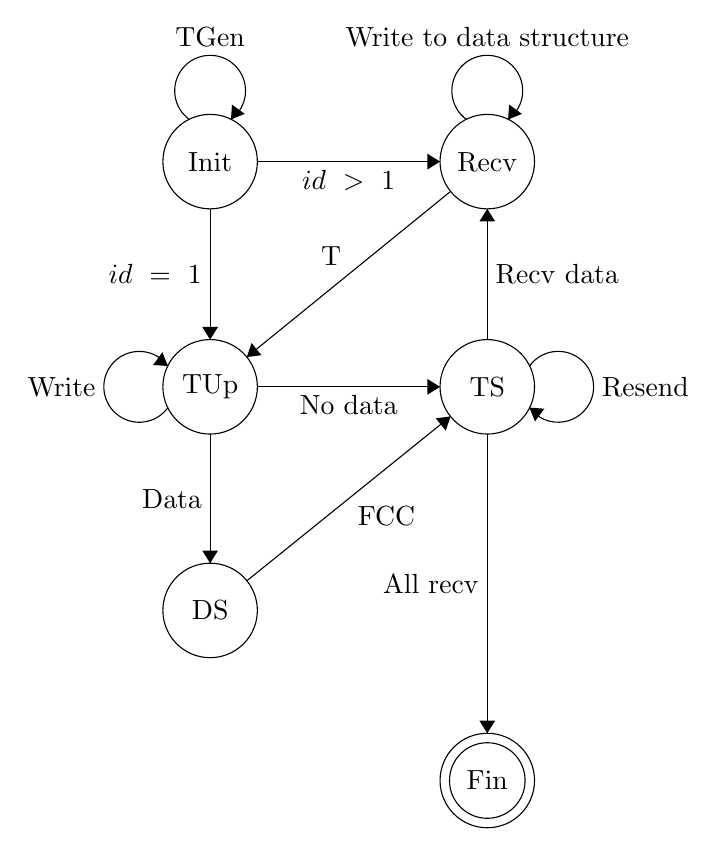
\begin{tikzpicture}[scale=0.2]
\tikzstyle{every node}+=[inner sep=0pt]
\draw [black] (21.4,-11.2) circle (3);
\draw (21.4,-11.2) node {$\mathrm{Init}$};
\draw [black] (21.4,-25.5) circle (3);
\draw (21.4,-25.5) node {$\mathrm{TUp}$};
\draw [black] (39,-11.2) circle (3);
\draw (39,-11.2) node {$\mathrm{Recv}$};
\draw [black] (39,-25.5) circle (3);
\draw (39,-25.5) node {$\mathrm{TS}$};
\draw [black] (21.4,-39.7) circle (3);
\draw (21.4,-39.7) node {$\mathrm{DS}$};
\draw [black] (39,-50.5) circle (3);
\draw (39,-50.5) node {$\mathrm{Fin}$};
\draw [black] (39,-50.5) circle (2.4);
\draw [black] (18.72,-26.823) arc (-36:-324:2.25);
\draw (14.15,-25.5) node [left] {$\mathrm{Write}$};
\fill [black] (18.72,-24.18) -- (18.37,-23.3) -- (17.78,-24.11);
\draw [black] (21.4,-28.5) -- (21.4,-36.7);
\fill [black] (21.4,-36.7) -- (21.9,-35.9) -- (20.9,-35.9);
\draw (20.9,-32.6) node [left] {$\mathrm{Data}$};
\draw [black] (24.4,-25.5) -- (36,-25.5);
\fill [black] (36,-25.5) -- (35.2,-25) -- (35.2,-26);
\draw (30.2,-26) node [below] {$\mathrm{No\ data}$};
\draw [black] (23.73,-37.82) -- (36.67,-27.38);
\fill [black] (36.67,-27.38) -- (35.73,-27.5) -- (36.36,-28.28);
\draw (32.6,-33.09) node [below] {$\mathrm{FCC}$};
\draw [black] (39,-22.5) -- (39,-14.2);
\fill [black] (39,-14.2) -- (38.5,-15) -- (39.5,-15);
\draw (39.5,-18.35) node [right] {$\mathrm{Recv\ data}$};
\draw [black] (36.67,-13.09) -- (23.73,-23.61);
\fill [black] (23.73,-23.61) -- (24.66,-23.49) -- (24.03,-22.72);
\draw (29.08,-17.86) node [above] {$\mathrm{T}$};
\draw [black] (21.4,-14.2) -- (21.4,-22.5);
\fill [black] (21.4,-22.5) -- (21.9,-21.7) -- (20.9,-21.7);
\draw (20.9,-18.35) node [left] {$id\mbox{ }=\mbox{ }1$};
\draw [black] (24.4,-11.2) -- (36,-11.2);
\fill [black] (36,-11.2) -- (35.2,-10.7) -- (35.2,-11.7);
\draw (30.2,-11.7) node [below] {$id\mbox{ }>\mbox{ }1$};
\draw [black] (37.677,-8.52) arc (234:-54:2.25);
\draw (39,-3.95) node [above] {$\mathrm{Write\ to\ data\ structure}$};
\fill [black] (40.32,-8.52) -- (41.2,-8.17) -- (40.39,-7.58);
\draw [black] (41.68,-24.177) arc (144:-144:2.25);
\draw (46.25,-25.5) node [right] {$\mathrm{Resend}$};
\fill [black] (41.68,-26.82) -- (42.03,-27.7) -- (42.62,-26.89);
\draw [black] (20.077,-8.52) arc (234:-54:2.25);
\draw (21.4,-3.95) node [above] {$\mathrm{TGen}$};
\fill [black] (22.72,-8.52) -- (23.6,-8.17) -- (22.79,-7.58);
\draw [black] (39,-28.5) -- (39,-47.5);
\fill [black] (39,-47.5) -- (39.5,-46.7) -- (38.5,-46.7);
\draw (38.5,-38) node [left] {$\mathrm{All\ recv}$};
\end{tikzpicture}
\caption{A general state machine for the program. T is for token, D is for data, S is for send,.}
\end{figure}

\subsection{Algorithm}
We dedicate a section to explaining the details of the protocol. As stated before, the protocal is split into three main parts: startup, message transmission, termination.

The startup is difficult because we must find a way to successfully establish the ring through which the token is passed (using unicast). Our approach to this is a simple ack routine. Every machine starts out by multicasting its own information so that everyone (ncluding the target) receives the information. In the meantime, every machine also filters through the received packets, looking for its target (the machine with the next sequential ID). Once it successfully receives the information, it sends a message to the target so the target knows to stop. If the machine receives conformation, then it sends a message to machine 1 (who is essentially the controller). Until all machines are done, machine 1 will not create the token therefore the transmission process will not start. Once all acks are received, the process starts with machine 1 sending data (note, once the other machines start receiving data packets, they know for sure that they're in the messaging stage).

The transmission proceeds as discussed in the introduction essentially covers everything. A note is that flow control is determined by how often various limits are reached. For example, if the rtr ever reaches a state of being completely full, then we lower the fcc meaning that people must send less (giving more opportunitites time for the machines to catch up).

Finally, termination is done by sending a mass of tokens before finaly closing. That way the probability of none of them being received is 0 in a practical setting.

\section{Results}
\begin{figure}[h]
\centering
\includegraphics[width=\linewidth]{benchmark1ex2}
\caption{Inital benchmark results. The y-axis is the number of seconds for transmission and the x-axis is the loss rate which goes from 0\%, 1\%, 2\%, 5\%, 10\%, 20\%.}
\end{figure}

\begin{figure}[h]
\centering
\includegraphics[width=0.5\linewidth]{chart1ex2}
\caption{Hard results.}
\end{figure}

\section{Conclusion}
TBD
\section{Discussion}
TBD
\end{document}

    Status
    API
    Training
    Shop
    Blog
    About

    © 2014 GitHub, Inc.
    Terms
    Privacy
    Security
    Contact

